\documentclass{article}
\usepackage[utf8]{inputenc}
\usepackage{float}
\usepackage{graphicx}
\usepackage{geometry}
\usepackage{tabularx}
\usepackage{acronym}
\usepackage{listings}
\usepackage{lmodern}
\usepackage[version=4]{mhchem}
\usepackage{multicol}
\usepackage{xcolor}

\title{Systems Integration - Assignment \#2}
\date{2019/2020}

\author{João Moreira - 2015230374 \\ 
João Soares - 2009113071 }

\renewcommand{\baselinestretch}{1.3}

\begin{document}

\maketitle

\section{Introduction}

\qquad The intent of this assignment is to develop a web application to manage an online store os secondhand items, called MyBay and deploy it using WildFly Application Server. In order to develop this application, we build a Maven architecture and used \ac{Java EE} and divided the system into three layers: presentation, business and data.

\section{Presentation layer}

\qquad To develop the presentation layer we used \ac{JSF} because it is a MVC (model, view, control) framework.

\qquad The passwords in this layer go always through MD5 encryption when they are inserted, only after this they are sent to the server. This prevents attacks that display the password to the attacker in plain text.

\qquad A none logged in user can go to the landing page, in this case the login, and access the sign up page, so he sign up and latter login to see the contents of the web-page. After logging in, the user is presented with the home page (figure 1). All of the pages, from this point forward, use a template that we created so that they can have the same header, giving access to the user to the home page, add item page, profile page and logout option anywhere on the system. 

\begin{figure}[H]
    \centering
    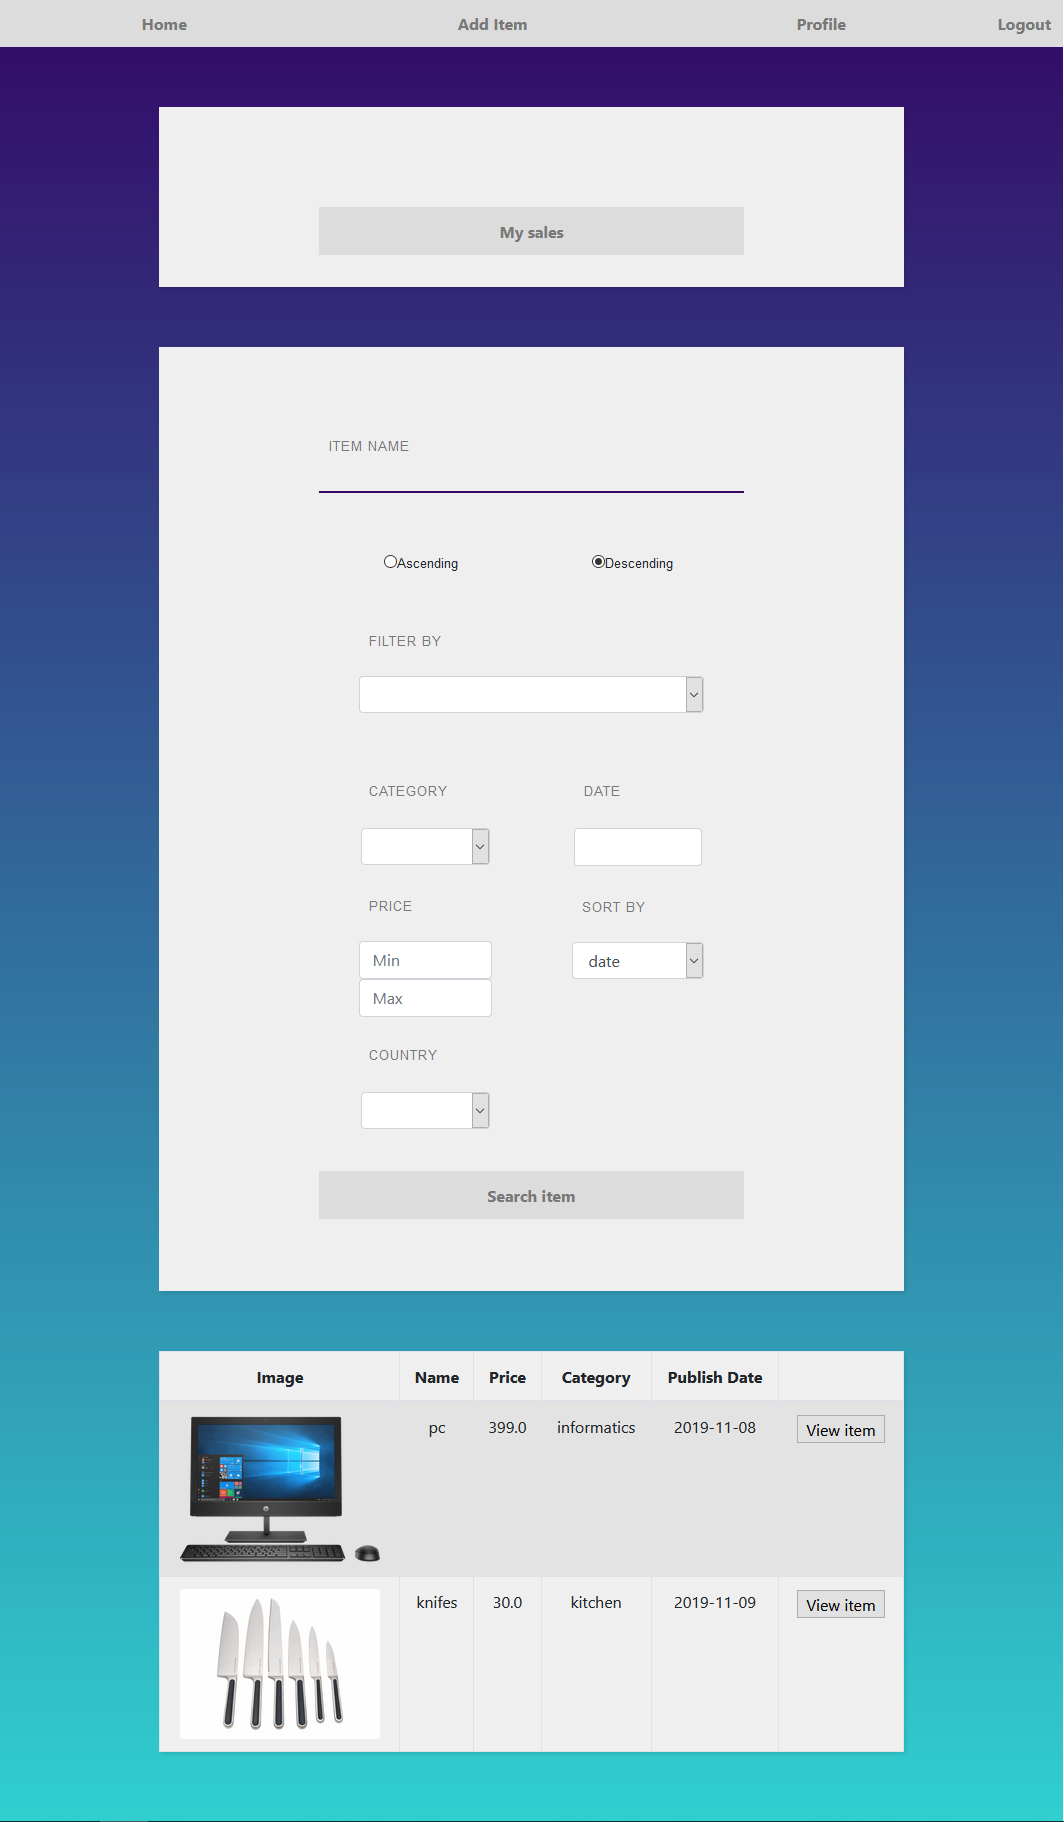
\includegraphics[scale=0.20]{homePage.png}
    \caption{Home page layout }
    \label{fig:homePage}
   \end{figure}

\qquad In the home page is where the user makes his searches. He's able to search for all items, by simply pressing the Search item button, he can see his own items, with the button my sales and can create various searches by using the input boxes, buttons and drop-down menus.

\qquad The add item section is the place where a new item can be created, and after that, by searching for his own sales, and clicking the view item button, the user can edit and delete his items.

\qquad In the profile area, the user can edit it's own name, country and password, as well as delete his account, deleting also his items for sale.

\qquad By logging out, the session is invalidated, so that the user needs to login again to see all of the pages above. 

\qquad One of the most challenging parts of the interface's implementation was the search part. We wanted to make it obvious to the user how the categories to search by are selected, so we made a drop-down menu where the user selects the category he wants to search by. E.g.: I only want to see the items in the category wc. To do that, I need to click filter by, select categories and in the categories drop-down menu select the category wc. After this, I press Search item and will get all items in this category.





\section{Business layer}

\qquad The connection to the data layer is performed by the business layer, whom has two local stateless \ac{EJB}s implemented. The account and sale. They are local because they are running in the same \ac{JVM} as the rest of the system and stateless sense we don't need to maintain a conversational state, we only need to perform simple operations. The transactions for this beans are managed by the container, although we don't make any transactions on this layer, hence the transactions to the database are handled on the level of the data layer.

\qquad On the AccountEJB, most of the information that goes to the presentation layer is boolean, sense the operations mainly need confirmations on said layer, exceptionally on the login, where we send a User class, created for this purpose, containing the information's about the user logged in (name, email, encrypted password and country).

\qquad The operations performed by this \ac{EJB} are sign up, login, update account and delete account. This operations send to the data layer a User class with only the information needed. In the sign up it sends a fully created user (name, email, password and country), in the case of the login just the email and password. For updating and removing the account the email is obligatory, although the update can bring a new name, country or password.

\qquad The SaleEJB, just like the AccountEJB, gathers booleans from the data layer, although, instead of User classes it collects Item classes to send to the presentation layer, and sends the mapped information to the presentation layer. The operations performed are create, list, update and delete sales, list an users items for sale and search sales. 





\section{Data layer}

\qquad The data layer works atop a database and exposes CRUD functionalities for the \ac{EJB}s ItemEJB and UserEJB. The database interactions use two other entities to be performed, PersistenceUser and PersistenceItem.  We can see how they interact in the following \ac{ER} (figure 2).

\begin{figure}[H]
 \centering
 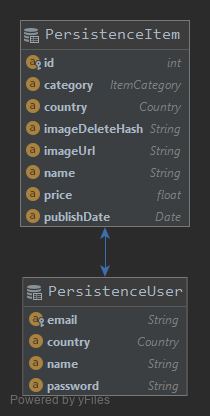
\includegraphics[scale=0.4]{ER_MyBay.png}
 \caption{MyBay \ac{EJB} \ac{ER} diagram }
 \label{fig:er}
\end{figure}

\qquad Both \ac{EJB}s interface extends the crudable interface and the ItemEJB's extends Searchable, meaning they both implement create, read, update and delete, while user also implements a listing of the user's items for sale and the item implementing a search method that has parameters as it's input.




\section{Project management and packaging}

\qquad The project is divided into 7 folders common, data, common\_data, business, common\_business, web and ear. The common folder has support functions, such as enumerations, converters from and to enumerations and types, it's here where we have the Item and User class used to transfer data between layers. The common\_data and common\_business it where we store the interfaces of the \ac{EJB}s of each layer. In the common\_data we also have the Crudable and Searchable interface. The web, data and business store each of our layers. The ear folder has the pom file that creates the deployable file, packaged has an ear file.

\qquad For logging we used the tool \ac{SLF4J}

\qquad Each of our folders has a pom fille. The root pom file has the modules of the project and the dependencies for the project, as well as the WildFly plugin configurations for the server that we're running WildFly on. The web pom has the URL where the system will be accessible from. The rest of the pom filles are used to define the packaging of the modules they're in, in this case both business and data are packaged has ejb, the web module is a war file and the common folders are jar files.\newline\newline






\textbf{Acronym list:}

\begin{acronym}
\acro{JVM}{Java Virtual Machine}
\acro{Java EE}{Java Enterprise Edition}
\acro{JSF}{JavaServer Faces}
\acro{EJB}{Enterprise JavaBeans}
\acro{JPA}{Java Persistence API}
\acro{JPQL}{Java Persistence Query Language}
\acro{ORM}{Object/Relational Mapping}
\acro{SLF4J}{Simple Logging Facade for Java}
\acro{ER}{Entity-Relationship}
\end{acronym}

\end{document}
